% ============================================================================
%  Beauty Filters Are a Third Class -- concise revision 2026-09-07.
%  Every number is traceable to a file under results/. No estimates.
% ============================================================================
\documentclass[conference]{IEEEtran}
\IEEEoverridecommandlockouts
\usepackage{cite}
\usepackage{amsmath,amssymb,amsfonts}
\usepackage{graphicx}
\usepackage{booktabs}
\usepackage{multirow}
\usepackage{xcolor}
\usepackage{url}
\usepackage{siunitx}
\usepackage[hidelinks]{hyperref}
\graphicspath{{figs/}}
\newcommand{\ours}{\textsc{Ours}}
\newcommand{\win}[1]{\textbf{#1}}

% Float placement. The defaults refuse a double-column float taller than 0.7 of the page,
% which pushed the two large evidence figures onto float pages *after* the bibliography and
% dragged the following floats with them (floats are placed first-in-first-out). Raising the
% fractions lets a tall figure* sit at the top of a text page. \raggedbottom then stops
% \flushbottom from stretching the space between paragraphs on pages that carry a float,
% which is what opened the gaps mid-column. Drop the \raggedbottom line if flush columns are
% required.
\renewcommand{\dbltopfraction}{0.92}
\renewcommand{\dblfloatpagefraction}{0.75}
\renewcommand{\topfraction}{0.92}
\renewcommand{\bottomfraction}{0.70}
\renewcommand{\textfraction}{0.06}
\renewcommand{\floatpagefraction}{0.75}
\setcounter{dbltopnumber}{3}
\setcounter{topnumber}{3}
\setcounter{totalnumber}{4}
\raggedbottom

\begin{document}

\title{Beauty Filters Are a Third Class:\\
Filter-Aware Face Manipulation Detection on Edge Devices}

\author{\IEEEauthorblockN{Qin-Ying Lin, Bo-Rong Chen, Chen-Shan Yu}
\IEEEauthorblockA{\textit{Advisor: Prof. Shang-Hong Lai}\\
\textit{National Tsing Hua University}}}

\maketitle

\begin{abstract}
Face manipulation detectors are trained as binary real-versus-fake classifiers, but a large
share of real-world face images are neither: they are genuine photographs with a beauty filter.
We show this omission is a structural defect, not a detail. On identical images at a matched
operating point, four ordinary beauty filters raise the false-accusation rate of \emph{every}
published detector that can be operated at that point (ten of eleven; the eleventh saturates)
from below 5\% to 22.5--33.7\%. A detector that treats filtering as its own class reaches
1.2\% (3/249; 0.0\%, 95\% upper bound 1.5\%, in the variant without the rendering
randomisation described below); the same architecture trained the conventional binary
way fails at 23.3\% on the standard forgery corpus and at 37.8\% on our own corpus, so the
cause is the label space, not the model or the data. A controlled experiment in which only
the label space varies shows that no threshold on any binary model matches the three-way
model on both safety axes, although the permissive binary variant (filters labelled
\emph{real}) comes within noise on one of them. We then locate the boundary of that fix, and it is not
where it appears to be: on 12{,}000 faces beautified by eight real Instagram filters a detector
trained on our own filters recognises 0.45\% as filtered and calls 94.4\% fake, yet a pre-registered
leave-one-filter-out experiment that holds the corpus fixed recognises an \emph{unseen} filter
algorithm at \textbf{94.3\%}, while training on a different corpus transfers at 1.41\%.
Changing the filter costs almost nothing; changing the rendering pipeline costs everything ---
so what a filter-aware detector needs is coverage of the deployment domain, not of every
filter. Acting on that diagnosis, we randomise the rendering pipeline during training instead
of collecting it, using no data from the target platform: real-filter recognition rises from
0.45\% to 29--33\% across three seeds, and to \textbf{13.3\%} at the deployed operating point
that keeps every release gate, for which the false-accusation rate above is the price.
We release the first same-protocol, filter-aware benchmark of published detectors
(13 models, 13{,}026 images, cluster-bootstrap intervals) and a 5.06\,M parameter hierarchical
detector that runs in \SI{43}{\milli\second} on a desktop CPU and \SI{0.1}{\second} in a phone
browser.
\end{abstract}

\begin{IEEEkeywords}
face forgery detection, beauty filters, retouching, explainability, edge deployment
\end{IEEEkeywords}

% ============================================================================
\section{Introduction}
% ============================================================================
\textbf{Problem.} Forgery detection is posed as \emph{real} versus \emph{fake}. Beauty
% !! 2026-09-13 FACTUAL ERROR, pending decision: the project's `face_reshaping` warp WIDENS
% faces by ~6% (True Test 62/62 pairs, training 60/60), it does not slim them. See
% results/research/face_reshaping_direction_audit_20260913/FINDINGS.md. Wording below must change.
filters --- skin smoothing, whitening, eye enlargement, face slimming --- are applied by
ordinary users to their own photographs; they change pixels while preserving identity. A
binary detector has to put them somewhere, and both choices are wrong: \emph{real} concedes
that edited pixels are invisible, \emph{fake} accuses the user of forgery. Saeed
\emph{et al.}~\cite{saeed2025} showed filters can hide fakes. The converse harm --- filters
causing genuine faces to be accused --- had not been measured.

\textbf{Finding.} It is universal. Every published detector we tested that can be operated at
a 5\% clean-real FPR --- ten of eleven, from 17.6\,M to 428\,M parameters, CNN or transformer,
forgery-corpus or self-blending training --- accuses 22.5--33.7\% of beautified genuine faces
at an operating point where it accepts 95\% of the same faces unfiltered
(Fig.~\ref{fig:teaser}, Fig.~\ref{fig:main}); the eleventh (NPR, 1.4\,M) saturates and has no
such operating point.

\textbf{Insight.} The failure is a property of the label space. A binary model has one
threshold, and a filter moves filtered genuine faces and filtered fakes in the \emph{same}
direction along it, so no threshold serves both. Adding \emph{filter} as a third class gives
the model somewhere to put the answer.

\textbf{Evidence.} Our own architecture trained the conventional binary way fails at 23.3\%;
trained three-way it reaches 1.2\% as deployed, and 0.0\% in the variant without rendering
randomisation. Four models identical in everything except label space
confirm that no binary variant, at any threshold, matches the three-way model on both axes
(Sec.~\ref{sec:necessity}).

\textbf{Boundary.} Real commercial filters bound the claim. On B-LFW --- 12{,}000 LFW faces
beautified by eight real Instagram filters --- a detector trained on our own filters recognises
0.45\% as filtered and
calls 94.4\% \emph{fake}. Two pre-registered experiments then separate the cause. Training on a
different corpus of real filters transfers at 1.41\%; a leave-one-filter-out experiment that
holds the corpus fixed recognises an unseen filter algorithm at 94.3\% (base-photo overlap
controlled). \textbf{The barrier is the rendering domain, not the filter algorithm}
(Sec.~\ref{sec:transfer}).

\textbf{Fix.} Because the barrier is a domain and not a vocabulary, it can be simulated rather
than collected. Randomising the rendering pipeline over \emph{all} classes during training lifts
real-filter recognition to 29--33\% (three seeds) with no target-platform data, and to 13.3\% at
the operating point that holds every release gate; this configuration is the deployed detector,
and it pays for the gain with the 1.2\% false-accusation rate quoted above (Sec.~\ref{sec:transfer}).

\begin{figure*}[t]
\centering
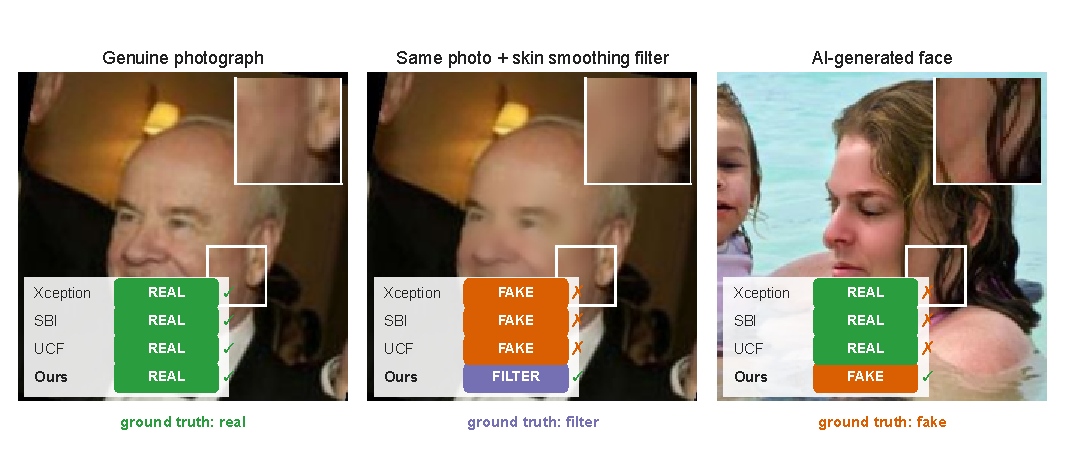
\includegraphics[width=\textwidth]{fig_teaser.pdf}
\caption{\textbf{The failure this paper measures.} A genuine face, the same face after a
skin-smoothing filter, and an AI-generated face, with the verdicts of three published binary
detectors and ours, all at a matched 5\,\% FPR on clean genuine faces. The binary detectors
accept the genuine face, accuse it once beautified, and miss the generated face; the
three-way detector answers \emph{filter} and \emph{fake}. Held-out True Test images; verdicts
verbatim from the released per-image scores. The pair is the first in the split on which all
three binary detectors flip: an illustration, not a sample; the rates are in
Table~\ref{tab:main}.}
\label{fig:teaser}
\end{figure*}

\textbf{Contributions.}
\begin{enumerate}
\item The first measurement of filter-induced false accusation, on identical images with
      confidence intervals, across eleven published detectors (Sec.~\ref{sec:p3}).
\item A controlled proof that a third class is \emph{necessary}: no binary label space
      reaches the three-way model on both safety axes (Sec.~\ref{sec:necessity}), and the cost
      of that class measured under the standard protocol (Sec.~\ref{sec:cost}).
\item An identification of what actually limits the fix. Two pre-registered experiments
      separate the filter algorithm from the corpus: holding the corpus fixed, an unseen
      filter algorithm is recognised at 94.3\% (three seeded folds, base-photo overlap
      audited and controlled); changing the corpus drops transfer to 1.41\%. Filter-aware
      detection needs coverage of the deployment domain, not of every filter
      (Sec.~\ref{sec:transfer}).
\item A deployable three-way detector with a structured explanation: 5.06\,M parameters,
      \SI{43}{\milli\second} on a desktop CPU and \SI{61}{}--\SI{103}{\milli\second} in the
      browser on two phones, made exportable by rewriting the spectral branch as a constant
      matrix product (Sec.~\ref{sec:system}, \ref{sec:deploy}).
\item A released benchmark (13 models, 3 protocols, per-image scores) and an honest account of
      where we lose (Sec.~\ref{sec:lose}).
\end{enumerate}

% ============================================================================
\section{Related Work}
% ============================================================================
\textbf{Binary detectors.} Xception on FaceForensics++~\cite{rossler2019} is the reference;
F3Net~\cite{qian2020}, SPSL~\cite{liu2021} and SRM~\cite{luo2021} add frequency cues,
RECCE~\cite{cao2022} reconstruction, UCF~\cite{yan2023ucf} disentanglement,
CORE~\cite{ni2022} consistency. SBI~\cite{shiohara2022} trains on self-blended reals only;
UnivFD~\cite{ojha2023} and NPR~\cite{tan2024} target generator-agnostic cues. None has a
class for identity-preserving retouching; we evaluate all of them.

\textbf{Prior art we do not claim.} Hierarchical decomposition of face manipulation is not
new. DAD-HCNN~\cite{jain2020} cascades original-vs-altered, then retouched-vs-GAN, then which
GAN, six years before this work, building on the same group's earlier
two-way detector~\cite{jain2018}; FALdetector~\cite{wang2019} detects and even partially
inverts Photoshop's geometric warping, which is our reshaping and eye-enlarging operations;
DFFD~\cite{dang2020} includes 18{,}416 FaceApp images. ForgeryNet~\cite{he2021} ships an
official three-way protocol, and TFMD~\cite{tfmd2023} is titled ``three-classification face
manipulation detection''. We claim none of these. What separates our setting is what the
third class \emph{contains}: ForgeryNet's identity-remained class is GAN semantic attribute
editing and TFMD's third class is reenactment, neither of which is cosmetic retouching;
DFFD's FaceApp images are attribute swaps (age, gender, glasses), not smoothing or slimming,
and its protocol is binary; DAD-HCNN's retouching comes from a single tool and its
cross-algorithm behaviour is never tested. Our contribution is the measurement of what
omitting cosmetic retouching costs a detector, and the evidence that the cost is structural.

\textbf{Retouching.} RetouchingFFHQ~\cite{ying2023} defines the four operations we use, and
its own cross-API table is the closest external evidence for our central limitation: transfer
from one commercial retouching API to another collapses its Sum-TP from 0.931 to 0.196, with
photometric filters (smoothing 0.086, whitening 0.041) failing far worse than geometric ones.
Its successor~\cite{liu2025} responds with a mixture of experts, one per retouching type plus
a shared expert --- an admission from the dataset's own authors that a single model does not
cover the space. Rathgeb \emph{et al.}~\cite{rathgeb2020} is the one prior work claiming
cross-tool robustness, under a leave-one-app-out protocol over six commercial beauty apps,
but their detector is differential: it needs a trusted reference image of the same person,
which a single-image forensic setting does not have.

\textbf{Filters as an attack.} Three recent works measure filters in the opposite direction to
ours: Libourel \emph{et al.}~\cite{libourel2024} build Celeb-DF-B and report video AUC drops
of about 0.15 across three detectors; Concas \emph{et al.}~\cite{concas2025} decompose the
attack asymmetrically and report VGG19's APCER rising from 30.1\% to 48.4\% under a smoothing
filter; Saeed \emph{et al.}~\cite{saeed2025} report attack success up to 64.63\%. All three
state mitigation as future work. We measure the converse harm --- filters causing genuine
faces to be accused --- and place filtering inside the label space rather than treating it as
an external perturbation.

\textbf{Lightweight detection.} MesoNet~\cite{afchar2018} (27{,}977 parameters) and
DefakeHop++~\cite{chen2022} (238\,K) are the reference points for small detectors, but neither
reports a model size or a latency on any device, which is the gap between ``few parameters''
and ``deployable''. DeFakeQ~\cite{li2026} is the one work we found with a real phone
measurement (\SI{31.8}{\mega\byte}, \SI{25}{\milli\second} per frame on Android), at a cost of
9.4 AUC points to quantisation; our export is lossless on decisions but larger and slower.

\textbf{Explanation.} FakeShield~\cite{xu2025} and FakeVLM~\cite{wen2025} explain with
multimodal LLMs at 7\,GB and ten seconds per image, far from edge use.
X$^2$-DFD~\cite{chen2025} is the closest relative of our evidence path: it feeds the output of
dedicated low-level artifact analysers into the explanation rather than letting the language
model free-generate. Saliency is cheap but Adebayo \emph{et al.}~\cite{adebayo2018} show it
can be insensitive to the model; we run that check on ourselves and fail it
(Sec.~\ref{sec:xai}).

% ============================================================================
\section{System}
\label{sec:system}
% ============================================================================
\begin{figure*}[t]
\centering
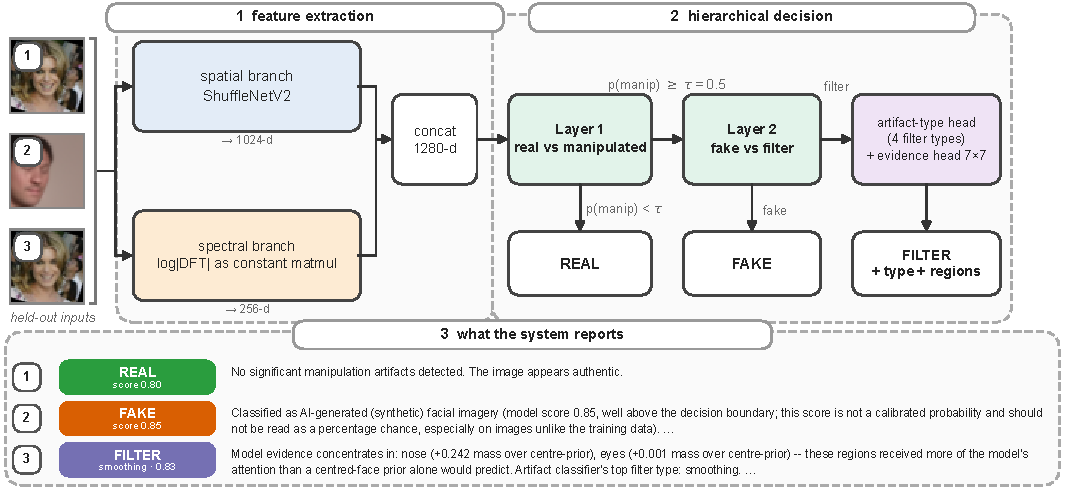
\includegraphics[width=\textwidth]{fig_pipeline.pdf}
\caption{\textbf{System overview, traced on three held-out inputs.} A spatial and a spectral
branch feed an explicit-threshold hierarchy: real versus manipulated, then fake versus filter,
then the filter operation; a patch evidence head produces region claims after subtracting a
centre-prior baseline. Panel 3 is what the system actually emitted for inputs 1--3: the chips
and the sentences are verbatim fields of the output record, abridged at a sentence boundary
where marked ``\ldots''. Inputs 1 and 3 are the same photograph without and with a beauty
filter. The DFT is exported as a constant matrix product so the graph runs on mobile runtimes
(Sec.~\ref{sec:deploy}).}
\label{fig:arch}
\end{figure*}

Fig.~\ref{fig:arch} is the whole system. \textbf{Classes} are semantic: \emph{real}
(unmodified), \emph{fake} (identity replaced or synthesised, including reenactment),
\emph{filter} (identity-preserving beautification). A commercial app that uses a neural network
internally still produces \emph{filter}.

\textbf{Backbone.} Filters attenuate high-frequency texture and shift colour without moving
geometry, so we pair a spatial stream with a spectral one:
\begin{equation}
\mathbf{f}(X) = \big[\,\mathrm{ShuffleNetV2}(X)\;\|\;\mathrm{CNN}_3\!\big(\log|\mathcal{F}(X)|+\epsilon\big)\,\big]
\in \mathbb{R}^{1280},
\end{equation}
with the two branches contributing 1024 and 256 dimensions and $\mathcal{F}$ the shifted
2-D DFT. The spatial--spectral pairing is a 2020-era pattern~\cite{qian2020,liu2021} kept for
its edge budget, not claimed as novel. ShuffleNetV2 was picked on Table~\ref{tab:backbone},
where all four candidates sit within 0.0006 AUROC, so the choice was effectively made on
memory; Section~\ref{sec:cost} revisits it.

\textbf{An exportable spectral branch.} Writing $\mathcal{F}$ with \texttt{torch.fft} makes
the model unloadable on mobile runtimes (Sec.~\ref{sec:deploy}). Because the input size is
fixed we evaluate the transform as a pair of constant matrix products,
$\mathcal{F}(X) = W_H X W_W / \sqrt{HW}$ with $W_H[k,m]=e^{-2\pi i km/H}$. Splitting
$W = C - iS$ into its cosine and sine parts and setting $P = C_H X$, $Q = S_H X$,
\begin{align}
\Re\,\mathcal{F}(X) &= P C_W - Q S_W, \label{eq:dftre}\\
\Im\,\mathcal{F}(X) &= -(P S_W + Q C_W), \label{eq:dftim}
\end{align}
so the branch needs four constant $224\!\times\!224$ matrices ($\approx$\SI{800}{\kilo\byte})
and six batched matrix products. The \texttt{fftshift} is folded into the constants by
rolling the rows of $W_H$ and the columns of $W_W$ by $N/2$, which costs nothing at
inference. The rewrite is exact, so existing weights are reused without retraining.

\textbf{Hierarchy.} Two binary heads share the features. Layer~1 gives
$p^{(1)}=(p_{\mathrm{real}}, p_{\mathrm{manip}})$ and Layer~2, applied to the same features,
gives $p^{(2)}=(p_{\mathrm{fake}\mid m}, p_{\mathrm{filt}\mid m})$. The three class
probabilities are the composite
\begin{equation}
P(\mathrm{real})=p_{\mathrm{real}},\quad
P(c)=p_{\mathrm{manip}}\cdot p_{c\mid m}\ \ \text{for } c\in\{\mathrm{fake},\mathrm{filter}\},
\end{equation}
which sums to one. The decision is \emph{not} an \texttt{argmax} over that vector, because
that would impose an implicit, image-dependent gate
$p_{\mathrm{manip}} > 1/(1+\max_c p_{c\mid m}) \in [0.50, 0.67]$. We use an explicit,
recorded threshold instead:
\begin{equation}
\hat{y}(X) =
\begin{cases}
\mathrm{real}, & p_{\mathrm{manip}} < \tau,\\[2pt]
\arg\max_{c} \; p_{c\mid m}, & p_{\mathrm{manip}} \ge \tau,
\end{cases}
\label{eq:rule}
\end{equation}
with $\tau = 0.5$, the published operating point. The deployed product and every evaluation
harness call this same function, so a reported number is the product's behaviour by
construction, verified on 13{,}244 dumped per-image decisions. For \emph{filter} an artifact
head then names which of the four operations was applied.

\textbf{Explanation.} The record carries class, operation, evidence regions, raw score and a
templated sentence. Regions come from a $7\times7$ patch evidence head trained on paired
pre/post-filter supervision, whose logits $z\in\mathbb{R}^{7\times7}$ are turned into a
normalised map $\hat{p} = \sigma(z)/\sum_{ij}\sigma(z)_{ij}$. A region $r$ (a group of cells:
eyes, nose, mouth, skin, contour) is reported only if it carries more probability mass than a
fixed centred-face prior $\pi$ would give the same region:
\begin{equation}
\Delta(r) = \sum_{(i,j)\in r}\hat{p}_{ij} \;-\; \sum_{(i,j)\in r}\pi_{ij}, \qquad
\mathcal{R} = \{\, r : \Delta(r) > 0 \,\},
\label{eq:region}
\end{equation}
reported in decreasing $\Delta$. Comparing \emph{mass to mass} rather than mean to mean is
what makes this size-neutral: regions differ in cell count by a factor of three, so a
mean-based score lets a small region win on a single peak while diluting a large one. $\pi$ is
the analytic mass of a centred Gaussian ($\sigma=56$\,px on the 224\,px frame) and does not
depend on the image, so $\Delta$ credits a region only for attention that centrality alone does
not already explain. If no region clears the prior, no region claim is made. Scores are
labelled as uncalibrated because calibration was tested and failed out of distribution.

\begin{table}[t]
\caption{Backbone selection, binary real vs.\ fake, identical training.}
\label{tab:backbone}
\centering\small
\begin{tabular}{@{}lcccc@{}}
\toprule
Model & F1 & AUROC & VRAM & Params \\
\midrule
MobileNetV4        & 0.9717 & 0.9981 & 0.55\,GB & 2.50\,M \\
EffNet-Lite0       & 0.9834 & 0.9981 & 1.69\,GB & 3.37\,M \\
ResNet18           & 0.9832 & 0.9984 & 1.10\,GB & 11.18\,M \\
\textbf{ShuffleNetV2} & \win{0.9837} & \win{0.9987} & \win{0.43\,GB} & \win{1.26\,M} \\
\bottomrule
\end{tabular}
\end{table}

% ============================================================================
\section{Benchmark}
% ============================================================================
\textbf{Training data.} \ours{} is trained on genuine faces (LFW, CelebA, AIGuard/real),
fakes (DeepFake-450K, DF40 diffusion/EFS methods, MidJourney) and filtered faces
(RetouchingFFHQ Megvii/Four variants plus our own four filter algorithms applied to genuine
faces). B-LFW, FairBeauty, the Alibaba variant of RetouchingFFHQ and Celeb-DF-B are held out
throughout and never enter training; every training split passes a content-hash contamination
audit against every evaluation set.

All models see identical image bytes and apply their own official pre-processing. Three
protocols: \textbf{P1}, 287 held-out generative fakes $\times$ 8 filter conditions (does a
filter let a fake escape?); \textbf{P2}, Celeb-DF-B~\cite{libourel2024}, 232 videos $\times$
4 commercial presets, third party, never trained on; \textbf{P3}, 249 genuine faces with our
four filters, paired with their 250 unfiltered sources (does a filter get a genuine face
accused?).

\textbf{Naming.} \ours{} always means the deployed detector of Section~\ref{sec:system}.
Everything else of ours is an experimental arm, named \emph{Arm-\ldots} and trained only to
isolate one variable; arms are never the proposed method and their numbers are not comparable
with \ours{} across protocols.

\textbf{Matched operating point.} Detectors publish thresholds calibrated on their own data,
so comparing them at those thresholds compares calibration, not behaviour. For a scorer
$s_m$ we therefore use the threshold that equalises the one quantity every detector should
agree on --- how often it accuses an \emph{unfiltered} genuine face:
\begin{equation}
t_m = \min\{\, t : \mathrm{FPR}_m(t) \le 0.05 \text{ on the clean real set} \,\}.
\end{equation}
At $t_m$ we then measure the two paired error rates
\begin{equation}
\mathrm{FA}_m = \Pr\!\big[s_m(x^{+}) \ge t_m\big], \qquad
\mathrm{MISS}_m = \Pr\!\big[s_m(x^{-}) < t_m\big],
\end{equation}
where $x^{+}$ is a \emph{filtered genuine} face and $x^{-}$ a \emph{filtered fake}. Intervals
are bootstrap 95\% CIs clustered by source image or video, $N_B=10{,}000$.

\textbf{The necessity criterion.} A filter displaces $x^{+}$ and $x^{-}$ in the \emph{same}
direction along any single score, so within a binary label space the two rates are coupled and
trading one against the other is all a threshold can do. We therefore do not compare our
operating point against each baseline's operating point, which would be a weak claim; we ask
whether \emph{any} threshold of \emph{any} binary model dominates ours. Writing
$(\mathrm{FA}^\ast, \mathrm{MISS}^\ast)$ for the three-way model, the three-way model is
undominated iff
\begin{equation}
\nexists\, m,\, t: \;\;
\mathrm{FA}_m(t) \le \mathrm{FA}^\ast \;\wedge\; \mathrm{MISS}_m(t) \le \mathrm{MISS}^\ast .
\label{eq:necessity}
\end{equation}
Section~\ref{sec:necessity} evaluates \eqref{eq:necessity} by sweeping $t$ over its full range
for all eleven published detectors and for three binary arms trained on our own data. It is an
empirical test over the models swept, not a theorem.

Every round reported here fixed its hypothesis, arms, metrics and verdict bars before any model
was trained or scored.

% ============================================================================

\section{Results}，
% ============================================================================
\subsection{Filters make every binary detector accuse genuine faces}
\label{sec:p3}
Table~\ref{tab:main} and Fig.~\ref{fig:main} are the main result. No published detector falls
below 22.5\% false accusation; \ours{} is 0.0\% (0/249; the bootstrap interval collapses on
a zero count, so we report the Clopper--Pearson 95\% upper bound, 1.5\%). Two facts about the
\ours{} row are stated rather than left implicit. First, it is read at the native
rule~\eqref{eq:rule}, where its clean-real FPR is 0.0\%, below the 5\% matched point; sweeping
its fake score to exactly 5\% FPR gives 2.0\% [0.9, 4.6] (Wilson), still an order of magnitude
below every baseline. Second, the third class is not free on clean faces: at the native rule
27.7\% of the 250 unfiltered genuine faces are routed to \emph{filter} (True Test real recall
72.3\% [66.4, 77.5]) --- a milder false claim, of retouching rather than forgery, which a binary
detector cannot make and which we report next to the 0.0\% rather than behind it. On cost we
are not uniformly smallest: we use 3.5--85$\times$ fewer parameters than the ten larger
baselines and are 2--28$\times$ faster than the nine slower ones, but NPR (1.44\,M,
\SI{23}{\milli\second}) and our own binary arm (2.53\,M, \SI{18}{\milli\second}) are both
smaller and faster --- the binary arm sits at the failing end of the safety axis, and NPR
cannot be operated at the matched point at all. The row that matters most is the second:
\emph{our} architecture under the conventional binary recipe fails at 23.3\%, indistinguishable
from the published detectors; the same architecture trained binary on \emph{our own} corpus
with the filter rows removed fails at 37.8\% (Table~\ref{tab:necessity}). Capacity,
architecture and corpus do not explain the failure; the label space does. For every published
detector, AUROC on \emph{filtered} fakes is higher than on unfiltered fakes: they detect the
filter, not the forgery.

\begin{table*}[t]
\caption{Cost and filter-aware safety on identical images (protocol P3). FA: fraction of 249
beautified genuine faces called \emph{fake}, threshold matched to 5\% FPR on the paired clean
reals, 95\% CI. CPU: desktop, batch 1, four threads, own pre-processing. AUROC: untreated
held-out generative fakes vs.\ 3{,}250 reals (P1).}
\label{tab:main}
\centering\small
\begin{tabular}{@{}clrrrcc@{}}
\toprule
Rank & Model (training data) & Params & MB & CPU ms & FA on beautified reals $\downarrow$ & AUROC \\
\midrule
% 2026-09-12: the deployed system now includes the rendering randomisation of
% Sec.~\ref{sec:transfer} (production v8.19-rr). Both configurations are reported
% because both were measured on these identical 13,026 images; the deployed one is
% the headline and the safer variant is disclosed directly beneath it.
1 & \textbf{\ours{}, three-way, deployed (ours)} & \win{5.06\,M} & \win{20.6} & \win{43} & \win{1.2\% [0.0, 2.8]} & \win{0.995} \\
-- & \quad\emph{same, without rendering randomisation} & 5.06\,M & 20.6 & 43 & 0.0\% [0.0, 1.5]$^{\ddagger}$ & 0.995 \\
\midrule
2 & UnivFD~\cite{ojha2023} (ProGAN)    & 427.62\,M & --    & 336  & 22.5\% [17.3, 27.7] & 0.588 \\
3 & \emph{Ours-arch, binary recipe} (FF++) & 2.53\,M & 10.3 & 18 & 23.3\% [18.1, 28.5] & 0.447 \\
3 & EfficientNet-B4 (FF++)              & 17.55\,M  & 71.0  & 891  & 23.3\% [18.1, 28.5] & 0.562 \\
5 & SPSL~\cite{liu2021} (FF++)          & 21.86\,M  & 87.8  & 181  & 24.5\% [19.3, 29.7] & 0.511 \\
6 & CORE~\cite{ni2022} (FF++)           & 21.86\,M  & 87.8  & 198  & 27.7\% [22.1, 33.3] & 0.494 \\
7 & F3Net~\cite{qian2020} (FF++)        & 22.52\,M  & 90.4  & 1187 & 28.5\% [23.3, 34.5] & 0.484 \\
8 & RECCE~\cite{cao2022} (FF++)         & 47.69\,M  & 191.5 & 755  & 28.9\% [23.3, 34.5] & 0.524 \\
8 & SRM~\cite{luo2021} (FF++)           & 55.35\,M  & 222.1 & 208  & 28.9\% [23.3, 34.5] & 0.699 \\
10 & Xception~\cite{rossler2019} (FF++) & 21.86\,M  & 87.8  & 710  & 29.7\% [24.1, 35.3] & 0.653 \\
11 & UCF~\cite{yan2023ucf} (FF++)       & 46.84\,M  & 188.0 & 310  & 32.1\% [26.5, 37.8] & 0.526 \\
12 & SBI~\cite{shiohara2022} (FF++)     & 17.55\,M  & 141.3 & 94   & 33.7\% [28.1, 39.8] & 0.631 \\
-- & NPR~\cite{tan2024} (ProGAN)        & 1.44\,M   & 17.4  & 23   & n/a$^{\dagger}$ & 0.450 \\
\bottomrule
\multicolumn{7}{@{}p{0.97\textwidth}@{}}{\footnotesize $^{\dagger}$ NPR has no 5\% FPR operating
point: it outputs a score of exactly 0 for 99.2\% of these 499 images, so a threshold at the
95th percentile of clean-real scores accuses every image (100\%) and the smallest threshold
with FPR $\le 5\%$ accuses 0.8\% at 0.8\% FPR and 3.5\% clean-fake recall; neither is a
comparable operating point, so NPR is excluded from the ranking. $^{\ddagger}$ Zero events: the
cluster bootstrap collapses to [0, 0]; the interval shown is the Clopper--Pearson 95\% upper
bound. Read at the native rule (clean-real FPR 0.0\%); at exactly 5\% FPR on the fake score
the rate is 2.0\% [0.9, 4.6]. UnivFD is distributed without a single archive; its parameters
are the CLIP ViT-L/14 it needs.}
\end{tabular}
\end{table*}

\begin{figure*}[t]
\centering
\includegraphics[width=\textwidth]{fig_main.pdf}
\caption{\textbf{Main result.} (a)~False accusation of 249 beautified genuine faces at a
matched 5\,\% clean-real FPR, 95\,\% cluster-bootstrap CIs. Our architecture under the binary
recipe (blue) fails like the published detectors; with a third class (green) it reaches
zero. (b)~The same models on the cost--safety plane; marker area scales with parameters.}
\label{fig:main}
\end{figure*}

\subsection{The third class is necessary}
\label{sec:necessity}
Within a binary label space, filters can go with \emph{real} or with \emph{fake}. We train
four models identical in backbone, data, recipe and seed that differ only in label space
(Table~\ref{tab:necessity}, Fig.~\ref{fig:ablation}a--b). Omitting filters gives 37.75\%
false accusation, inside the published band. Merging filters into \emph{fake} destroys the
forgery signal (clean fake recall 41\%). Merging into \emph{real} is the only sensible binary
option and it is close: the three-way model misses 1.57\,pp fewer filtered fakes
(CI $[-2.27,-0.92]$) and accuses 1.20\,pp fewer filtered reals (CI $[-5.62,+3.21]$,
directional only). The pre-registered test is stricter than these point estimates: sweeping
$t$ over its full range for every binary arm \emph{and} for all eleven published detectors,
criterion~\eqref{eq:necessity} is satisfied --- no threshold on any of the fourteen binary
models attains both a lower-or-equal $\mathrm{FA}$ and a lower-or-equal $\mathrm{MISS}$ than
the three-way model, and for every binary arm the gap on at least one axis excludes zero. At
its native rule~\eqref{eq:rule} the three-way model sends 94.78\% of filtered genuine faces to
\emph{filter} --- the answer a binary label space has no symbol for.

\begin{table}[t]
\caption{Four purpose-built arms, identical but for the label space, at 4.80\% clean-real FPR.
These are not \ours{}: they are retrained from scratch so that nothing but the label space
differs, which \ours{}' warm-start lineage would violate.}
\label{tab:necessity}
\centering\scriptsize
\begin{tabular}{@{}lccc@{}}
\toprule
Arm (label space) & FA & Miss & Clean fake \\
\midrule
\textbf{Arm-3way} & \win{8.84\%} & \win{1.97\%} & 98.61\% \\
Arm-filter$\rightarrow$real & 10.04\% & 3.54\% & 98.95\% \\
Arm-nofilter                & 37.75\% & 3.41\% & 98.61\% \\
Arm-filter$\rightarrow$fake & 41.37\% & 76.37\% & 41.11\% \\
\bottomrule
\end{tabular}\\[2pt]
\raggedright\scriptsize FA = false accusation of filtered reals; Miss = filtered fakes missed;
Clean fake = clean-fake recall.
\end{table}

\begin{figure*}[t]
\centering
\includegraphics[width=\textwidth]{fig_ablation.pdf}
\caption{\textbf{Ablations.} (a)~Full threshold sweep of every binary model in the
false-accusation / miss plane; three-way models (stars) lie below and left of every curve.
(b)~The four label spaces at the matched operating point. (c)~Cost of the third class under
the standard FF++ protocol, paired bootstrap on the difference. (d)~Backbone substitution on
the release gates: MobileNetV4 wins in-house filter recall and loses both external safety
gates.}
\label{fig:ablation}
\end{figure*}

\subsection{What actually blocks it: the corpus, not the filter}
\label{sec:transfer}
The obvious objection to Section~\ref{sec:p3} is that we generate the filters we are evaluated
on. We tested it on real ones. \textbf{B-LFW}~\cite{sanchez2022} applies eight real Instagram
beauty filters to 12{,}000 LFW faces. Trained only on our own filters, the detector recognises
\textbf{0.45\%} of them
as \emph{filter}, and calls \textbf{94.4\%} of these genuine faces \emph{fake} --- the very
harm this paper measures in others, at three times the worst published rate. (This is the
configuration analysed throughout this subsection; the randomisation introduced at its end is
what the deployed detector adds, and it raises the 0.45\% to 13.3\%.) On FairBeauty
(9{,}806 beautified FairFace images) it is 12.9\% filter and 63.1\% fake. A resolution control
separates the cause from the domain shift: the same 2{,}000 LFW originals downsampled to
B-LFW's 112\,px give 73.2\% \emph{filter} and 0.25\% \emph{fake}, so resolution alone moves
images towards \emph{filter}; it is the beautification on top of it that produces the
\emph{fake} verdict.

We then ran the fix a reviewer would ask for, pre-registered with bars set before training
(BUILD $\ge 50\%$, PARTIAL 10--50\%, REJECT $<10\%$): add a real commercial filter family
(8{,}828 FairBeauty images) to the Layer~2 filter class, holding everything else at the
production recipe, and test on the fully held-out B-LFW. The verdict is \textbf{REJECT}.
B-LFW moves from 0.45\% to \textbf{1.41\%} (Wilson CI [1.21, 1.64]), with all eight filters
below 2.6\% --- the failure is uniform, not a partial signal
(Fig.~\ref{fig:transfer}b). The training itself worked: the held-out, identity-disjoint
FairBeauty validation split moves from 12.9\% to \textbf{70.7\%}, and the algorithmically
generated Alibaba set stays at 97.7\%. All five release gates are unchanged, including the
composite-attack error ($+0.04$\,pp), so the filter class took no territory from the fake
class.\footnote{Gate deltas in this section are within-harness, and all rounds in this
subsection predate the rendering randomisation of Sec.~\ref{sec:transfer}, so their baseline is
the pre-randomisation configuration: its composite-attack error reads 2.80\% in
Sec.~\ref{sec:p1} and 2.84\% in the harness used for these two rounds --- 64 versus 65 of
2{,}289 images. We quote deltas rather than absolute values where the comparison is within a
harness.}

\begin{figure*}[t]
\centering
\includegraphics[width=\textwidth]{fig_transfer.pdf}
\caption{\textbf{The corpus binds, not the filter algorithm.} (a)~Adding one real commercial
filter family (FairBeauty) to Layer~2 training: the trained family is learned
(12.9$\to$70.7\%), an already-solved algorithmic family is unchanged (97.7\%), and the
held-out real family barely moves (0.45$\to$1.41\%); shaded bands are the bars declared before
the run. (b)~That failure is uniform across all eight Instagram filters, not a partial signal.
(c)~But changing the filter algorithm was never the problem. Holding the corpus fixed and
holding out one filter at a time, an unseen filter is recognised at 94.3\% (dots are the three
seeded folds, unseen base photographs only), against 1.41\% when the corpus changes instead.}
\label{fig:transfer}
\end{figure*}

That experiment, however, changes \emph{two} variables at once: the filter algorithms and the
corpus (FairFace versus LFW, different crops, resolution and rendering pipeline). Which one
binds? We separated them with a pre-registered leave-one-filter-out design on B-LFW itself,
holding the corpus fixed: train the same Layer~2 recipe on seven of its eight Instagram
filters, test on the eighth, with folds $\{1,3,7\}$ drawn by seed before any run.

One audit was necessary first, and it changed how we report the number. B-LFW applies several
filters to the same base photographs: 44.1\% of its images have a near-duplicate (64-bit dHash,
Hamming $\le 4$) under a \emph{different} filter id, with a spike at distance 0--2. A raw
held-out fold therefore mixes ``unseen filter on a photo I have seen'' with ``unseen filter on
a photo I have not seen''. We split every fold on that criterion (42.3--47.6\% seen-base) and
report both.

\begin{table}[t]
\caption{Leave-one-filter-out on B-LFW, corpus held fixed. Folds fixed by seed before
training. The last column is the honest cross-algorithm test.}
\label{tab:lofo}
\centering\scriptsize
\begin{tabular}{@{}lcccc@{}}
\toprule
Held-out filter & no B-LFW & all & seen base photo & \textbf{unseen base photo} \\
\midrule
filter 1 & 0.80\% & 91.81\% & 92.28\% & \win{91.46\%} [89.4, 93.2] \\
filter 3 & 0.53\% & 95.96\% & 95.68\% & \win{96.21\%} [94.6, 97.3] \\
filter 7 & 0.07\% & 95.69\% & 96.26\% & \win{95.27\%} [93.7, 96.5] \\
\midrule
mean     & 0.47\% & 94.49\% & 94.74\% & \win{94.31\%} \\
\bottomrule
\end{tabular}
\end{table}

The result is unambiguous (Table~\ref{tab:lofo}, Fig.~\ref{fig:transfer}c). An unseen filter
algorithm is recognised at \textbf{94.31\%} on base photographs the model has never seen, up
from a 0.47\% baseline --- and in all three folds the seen-base and unseen-base subsets are
statistically indistinguishable, so photo overlap does not explain it. The held-out filter even
lands at the same level as the seven trained ones (mean 94.5--95.2\%). Both pre-declared
controls hold: training worked, and the composite-attack error moves $+0.13$\,pp with True
Test and Alibaba recall unchanged, so the filter class took nothing from the fake class.

Placing the two experiments side by side gives the finding. Change the filter algorithm and
hold the corpus: \textbf{94.31\%}. Change the corpus: \textbf{1.41\%}. The binding constraint
is coverage of the \emph{rendering domain}, not coverage of filter algorithms. This corrects
the natural reading of the previous experiment --- that the model learns one filter family at a
time --- which was available only because that experiment moved both variables together. It
also explains the 94.4\% false-accusation rate we started this section with: B-LFW is
\SI{112}{px} MTCNN crops, a pipeline our production data never contains, and the resolution
control confirms the domain alone moves the model (the same LFW originals downsampled to
\SI{112}{px} flip 73.2\% to \emph{filter}).

The practical consequence is a cheaper requirement than ``collect every filter'': to deploy on
a platform, collect samples of \emph{that platform's rendering pipeline}.

\textbf{Randomising the rendering pipeline instead of collecting it.} If the rendering domain binds,
the domain can also be simulated. We re-train Layer~2 with one change: with probability $0.5$ every
training image, \emph{whatever its class}, passes through a random rendering pipeline --- crop jitter,
downscaling to 96--160\,px with a random resampler, JPEG at quality 50--95 with probability $0.7$, and
upscaling back to 224\,px. Because the pipeline is applied identically to fake and filter rows,
resolution, resampling and compression carry no label information, and the model has to key on the edit
itself. The only previous attempt to use post-processing in this project applied it to the
\emph{real} class alone and taught the model that low resolution means \emph{real}, which lowered B-LFW
recognition. No B-LFW, FairBeauty or Instagram image is used for training or for model selection
(Table~\ref{tab:renderrand}).

\begin{table}[t]
\caption{Rendering randomisation on Layer~2, zero-shot. Control = same epochs, no randomisation. Seed 3
is read at $\tau_{\mathrm{filter}}=0.72$, fixed before it was trained; all six release gates pass there.
\textbf{The seed-3 column is the deployed detector} and is the row reported as ours in
Table~\ref{tab:main}.}
\label{tab:renderrand}
\centering\scriptsize
\begin{tabular}{@{}lccc@{}}
\toprule
 & Control & Randomised (3 seeds) & Seed 3 @0.72 \\
\midrule
B-LFW recognised as \emph{filter} & 0.68\% & 29.2 / 33.0 / 30.5\% & 13.3\% \\
FairBeauty recognised as \emph{filter} & 26.5\% & 50.1 / 49.8 / 44.9\% & 33.6\% \\
AIGuard/unseen AUROC & 0.834 & 0.907 / 0.897 / 0.892 & 0.892 \\
Composite (fake+filter) error & 2.97\% & 5.46 / 5.55 / 4.28\% & 3.23\% \\
P3 filtered reals called \emph{fake} & 0.0\% & 0.0 (seed 1) & 1.2\% \\
\bottomrule
\end{tabular}
\end{table}

At the native threshold the randomised model recognises 29--33\% of B-LFW across three seeds, against
0.68\% for the control, with every one of the eight filters moving; FairBeauty rises from 26.5\% to
45--50\%, and AIGuard/unseen AUROC from 0.834 to 0.89--0.91. The gain is not an operating-point effect: at
the same safety constraint (composite error $\le 3.76\%$, clean fake recall $\ge 99\%$, filter recall
$\ge 90\%$) the control's best threshold recognises 1.8\% of B-LFW and the randomised model 14.5--21.7\% (three seeds).
It is not free either. Raising the Layer~2 threshold to meet the safety gates costs recall on the real
filters (13.3\% on the independent seed), and false accusation on our own filters rises from 0/249 to
3/249, while the composite in-house error rises from 2.80\% to 3.23\%. Both costs land inside the
incumbent configuration's own 95\% intervals (composite CI [1.92, 3.76]; the 0/249 has a
Clopper--Pearson upper bound of 1.47\%), whereas the gains lie far outside them and replicate on three
seeds, so \textbf{this configuration is the one we deploy}: the seed~3 column of
Table~\ref{tab:renderrand}, read at the threshold fixed before that seed was trained, is the system
reported as ours in Table~\ref{tab:main}. Two checks support the choice rather than the summary
statistics alone. First, on the only \emph{externally} sourced safety benchmark --- Celeb-DF-B, held
out and never trained on --- the beautified-deepfake escape rate is statistically unchanged
(23.38\% $\to$ 23.55\%, near-coincident intervals), so the cost is confined to our own composite
metric. Second, false accusation on \emph{clean} genuine faces improves (0.28\% $\to$ 0.12\%), and
across twenty perturbation conditions the trade-off is not amplified: the worst degradation is
0.8\,pp, genuine-face recall is identical in all twenty, and the two most degraded conditions ---
$k{=}9$ blur and $4\times$ downscaling --- \emph{improve} by 0.8 and 1.6\,pp in filter recall, which is
the direction the mechanism predicts.
A threshold of 0.61 also passes every gate and would recognise 21.7\% of B-LFW, but it was found by
reading the test-set frontier; we report it as a frontier point and do not operate there. The same randomisation applied to Layer~1 does \emph{not} stop downsampled genuine
photographs being routed to \emph{filter} (76.5\% vs.\ 73.8\%). A plausible reason, not tested here, is
that downscaling and skin smoothing are both low-pass operations and cannot be told apart at the pixel
level.

\subsection{Two costs of the design}
\label{sec:cost}
\textbf{The third class costs cross-dataset AUC.} Pairs of arms on FF++ frames, each pair sharing a
seed and differing only in whether 12{,}000 retouched images are added as a third class, over four
seeds: the third class costs $-0.014$ AUC on DFD (95\% $t$-interval over seeds $[-0.026,-0.003]$)
and $-0.012$ on Celeb-DF-v2 ($[-0.040,+0.016]$, not resolved), with in-domain F1 unchanged
(Fig.~\ref{fig:ablation}c). A single-seed version of this experiment had suggested $-0.037$ on
Celeb-DF-v2; that seed turned out to be the most extreme of four, which is why we report seeds as the
unit. We pre-registered the opposite hypothesis and it was refuted. The trade is explicit: zero false
accusation, and no binary equivalent, for about 1.4 points of zero-shot forgery detection.

\textbf{A stronger backbone does not buy the safety back.} MobileNetV4 in place of
ShuffleNetV2, everything else fixed, improves the matched frontier (false accusation
8.84$\to$2.81\%, CI excludes zero, replicated on a second seed) but fails the two release gates
that define this paper: composite fake-plus-filter error 11.4\% flat and 15.1\% hierarchical
against 2.8\%, third-party retouching recall 72\% and 57\% against 98\%
(Fig.~\ref{fig:ablation}d). \ours{} therefore stays on ShuffleNetV2: the property this paper is
about comes from the label space, not the backbone.

\subsection{Composite attack (P1)}
\label{sec:p1}
On 2{,}289 fakes with a filter applied, our end-to-end error is \win{3.23\%} [2.28, 4.26]
(2.80\% [1.92, 3.76] without rendering randomisation, which is where the 2.11\,pp
filter-attributable decomposition below was measured; the two intervals overlap). Published detectors cannot be ranked here: their
AUROC on the unfiltered sources is 0.45--0.70 against our 0.995, so matching recall pushes
them to 89--100\% FPR. FF++- and ProGAN-trained detectors do not transfer to this generative
family; we report that as scope, not as a win.

\begin{figure*}[!t]
\centering
\includegraphics[width=\textwidth]{fig_explain.pdf}
\caption{\textbf{What the system reports} on held-out images. One row per filter operation:
the genuine photograph, the filtered version, the amplified pixel difference the filter
introduced, the change in the log-magnitude spectrum, the evidence-head map, and the
structured explanation. Filters remove high-frequency texture (smoothing), shift luminance
(whitening) or warp geometry (eye, reshaping); the explanation names only regions that beat
a centre prior and reports measurements with their validated power. Each filter record also
ends with a caveat clause, identical in wording across the four rows and omitted here for
space: these measurements separate filtered from authentic faces at a single-image AUROC of
only 0.54--0.57, so the record reports them rather than asserting them as abnormal. The last
two rows are the other two classes. For \emph{fake} and \emph{real} no paired counterpart and no region-level
ground truth exist, so the system emits no difference map, no spectral pair and no region
claim --- the record's region list is empty by design. That is the explanation asymmetry
quantified in Sec.~\ref{sec:xai}, drawn rather than asserted.}
\label{fig:explain}
\end{figure*}

\subsection{Standard cross-dataset protocol}
\label{sec:crossdataset}
To be comparable with the literature we also train our architecture on FF++ c23 only and
score every model zero-shot on the same frames (Table~\ref{tab:crossdataset},
Fig.~\ref{fig:crossdataset}). SBI leads both corpora and lies outside our interval. Over five seeds
our 3.90\,M MobileNetV4 variant reaches $0.809$ $[0.786, 0.833]$ on Celeb-DF-v2 and $0.899$
$[0.879, 0.919]$ on DFD, statistically indistinguishable from Xception ($0.806$ / $0.901$) at
$5.6\times$ fewer parameters, above EfficientNet-B4, SPSL and UnivFD, and within the interval of
UCF, CORE and SRM. Per-seed values range over 4.4 points on the 389-frame Celeb-DF-v2 holdout, so
single-seed rankings on it are not meaningful. Our ShuffleNetV2 variant is 7--8 points below
Xception on Celeb-DF-v2. Two inconvenient facts: the production recipe scores
0.15--0.17 AUC below its FF++-trained sibling, so the deficit is training coverage, not
architecture; and the spatial-only variant beats the dual-branch one here, so the spectral
branch helps the filter task and low-FPR regime but not cross-dataset forgery detection.

\begin{table}[t]
\caption{All models trained on FF++ c23, zero-shot frame AUC on the same frames.}
\label{tab:crossdataset}
\centering\scriptsize
\begin{tabular}{@{}lrcc@{}}
\toprule
Model & Params & CDFv2 & DFD \\
\midrule
SBI~\cite{shiohara2022}     & 17.55\,M & \win{0.8928} & \win{0.9273} \\
Xception~\cite{rossler2019} & 20.81\,M & 0.8063 & 0.9007 \\
Ours, MobileNetV4           & 3.90\,M & 0.809$^{\ast}$ & 0.899$^{\ast}$ \\
Ours, ShuffleNetV2          & \win{2.55\,M} & 0.7278 & 0.8487 \\
Ours, spatial only          & \win{1.80\,M} & 0.7358 & 0.8602 \\
\emph{Ours, prod.\ recipe}  & 5.06\,M & 0.5794 & 0.6887 \\
\bottomrule
\multicolumn{4}{@{}p{0.95\columnwidth}@{}}{\footnotesize $^{\ast}$ mean of five seeds; 95\% $t$-intervals $[0.786, 0.833]$ and $[0.879, 0.919]$. CDFv2 = Celeb-DF-v2.}
\end{tabular}
\end{table}

\begin{figure}[t]
\centering
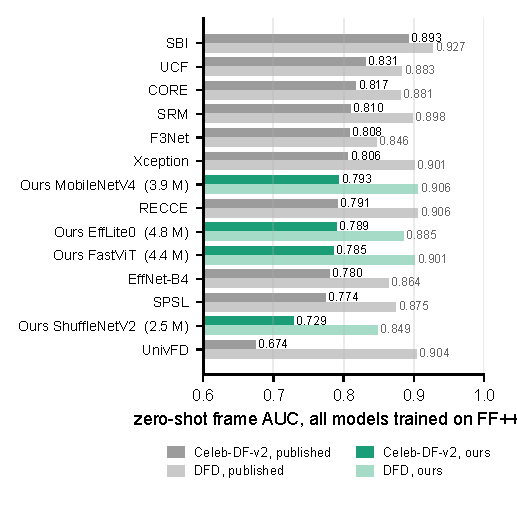
\includegraphics[width=\columnwidth]{fig_crossdataset.pdf}
\caption{\textbf{Standard protocol, same frames.} Published checkpoints (grey) were run by
us on our Celeb-DF-v2 (389 frames) and DFD (1{,}521 frames) holdouts. One seed per bar.}
\label{fig:crossdataset}
\end{figure}

\subsection{P2: where we lose}
\label{sec:lose}
On Celeb-DF-B (protocol P2) our beautified AUROC is 0.524 against 0.735--0.756 for Xception,
UCF and SBI; we are worse than nineteen of the twenty-one models scored on that axis.
The cause is not filter robustness: we call 86--88\% of \emph{untreated} Celeb-DF real frames
fake. Our real class is almost entirely photographs; adding FaceForensics++ real video frames
to training halves that rate (87.7$\to$41.7\%), while removing the 11{,}735 fakes derived from
Celeb-DF changes nothing ($-0.26$\,pp, CI $[-1.98,+1.47]$). The deficit is coverage of real
video frames. The same corpus-shortcut pattern recurs in two other components we tested --- a
7\,B vision-language teacher (99.7\% in-domain against 59.9\% on our held-out set) and the
artifact head across retouching algorithms --- and, given Section~\ref{sec:transfer}, we now
read all three as instances of one thing: these models key on the corpus that produced the
image. We treat it as a finding rather than a footnote: fluent or high in-domain performance
is no evidence of having learned the task.

\subsection{Explanation}
\label{sec:xai}
Fig.~\ref{fig:explain} shows the full record for four filtered faces. We report a null
result for saliency: production Grad-CAM++ is statistically indistinguishable from a fixed
centre-Gaussian prior under RISE deletion (AUC 0.787 vs.\ 0.787) and fails the Adebayo
randomisation check (Spearman 0.83--0.97), so we claim no faithfulness for heat-maps. The
patch evidence head beats the centre prior on independent ground-truth masks
(IoU@10\% 0.61 vs.\ 0.57, paired CI excludes zero) with an uneven margin by filter type; the
explanation reports only regions that clear that prior and states each measurement's
validated single-image power rather than asserting an abnormality.

The fake branch is thinner and we quantify how thin. Its text conditions only on a confidence
tier and one texture measurement --- two independent binary clauses, so at most four sentence
patterns are reachable at all; over the full True Test fake set (270 images, 267 predicted
fake) all four occur (68.9\% / 16.5\% / 9.7\% / 4.9\%), against 56 distinct explanations over 56
filtered faces. To close that gap we
distil a vision-language teacher's artifact vocabulary into a \textbf{35{,}854-parameter}
linear head on the frozen production features, changing no production weight. On a test set
that can measure all fourteen concepts it recovers ten of them at F1 0.73--0.96, including the
four filter operations (smoothing 0.96, whitening 0.85, reshaping 0.60, eye enlarging 0.52).
It nevertheless \emph{misses} its own pre-declared macro-F1 bar, 0.6843 against 0.70, because
two artifact concepts occur 6 and 54 times in the reference split; over the thirteen concepts
with support at least 50 it is 0.7361. And its filter concepts do not cross vendors: macro-F1
0.7396 within the trained family against \textbf{0.1416} on the third-party retouching set,
where \emph{whitening} fires on 0.2\% of positives and \emph{eye enlarging} fires on 99.8\% of
everything. Alibaba is a different vendor \emph{and} a different corpus, so this is the same
domain-coverage limit as Section~\ref{sec:transfer}, now visible in a component that shares no
weights with the classifier.

\subsection{Deployment}
\label{sec:deploy}
\texttt{torch.fft} exports to an operator mobile runtimes cannot parse, so the model did not
load at all. Equations \eqref{eq:dftre}--\eqref{eq:dftim} replace it with constant matrix
products: mathematically identical, no retraining, standard operators only. The fp32 export
reproduces the PyTorch decision on 769 of 769 held-out images; 8-bit quantisation is not
usable because the spectrum's $7.6\times10^{9}$ dynamic range collapses 98\% of bins. We
measured the four exported graphs (\SI{33}{\mega\byte}) in the browser on two phones
(Fig.~\ref{fig:ondevice}): an iPhone on iOS~26.2.1 takes \SI{75.9}{\milli\second} for the
real/fake route and \SI{103.4}{\milli\second} for the full filter record, and an Android
device on Chrome takes \SI{61.3}{} and \SI{83.7}{\milli\second}. Both run WebAssembly on a
single thread with no GPU, so these are upper bounds on a native build, which we did not
measure.

\begin{figure}[!t]
\centering
\includegraphics[width=\columnwidth]{fig_ondevice.pdf}
\caption{\textbf{On-device latency on two phones}, browser WebAssembly, one thread, no GPU;
mean of 50 runs after 5 warm-ups on a fixed input. Model sizes 10.96 / 10.96 / 5.05 /
6.06\,MB.}
\label{fig:ondevice}
\end{figure}

% ============================================================================
\section{Limitations}
% ============================================================================
\begin{itemize}
\item \textbf{Filter coverage.} The in-house false-accusation figures hold for four operations at
      one parameter setting each. Without rendering randomisation \ours{} recognises 0.45\% of
      B-LFW's real filters; the deployed detector, which includes it, recognises 13.3\% --- better
      by a factor of 30, but still a small minority of real commercial filters, and the safety
      gates rather than the mechanism are what cap it (29--33\% at the native threshold). The
      deployed configuration also has a single seed behind its operating point, and the
      configuration it replaced was never re-run with a second seed either.
\item \textbf{Clean-face cost of the third class.} The false-accusation metric counts only
      \emph{fake} verdicts. At the native rule \ours{} routes 27.7\% of clean True Test faces,
      15.3\% of 2{,}000 native-resolution LFW training reals and 73.2\% of the same reals
      downsampled to 112\,px to \emph{filter}. A binary detector cannot make this milder error;
      ours does, and it grows with any loss of resolution. The mild-filter versus
      post-processing boundary (JPEG, resizing, blur) is measured at AUROC 0.38--0.52 for
      three of our four operations, so ``filter'' partly means ``pixel statistics of a
      processed image'' rather than ``beautification''.
\item \textbf{Scope of the transfer result.} Three of eight folds, one seed; all eight filters
      come from one platform and plausibly share a rendering stack; training had already seen
      10{,}498 images of that domain. It says nothing about an unseen corpus. The seen/unseen
      split controls base photographs, not identities.
\item \textbf{Explanation.} No faithfulness is claimed for saliency; the fake branch composes
      four sentence patterns from two independent binary clauses; the tag head misses its own
      bar; no human study.
\item \textbf{Detection.} We trail SBI and Xception on the standard cross-dataset table, and
      the artifact head is weak across unseen retouching implementations.
\item \textbf{Backbone.} MobileNetV4 beats ShuffleNetV2 at forgery detection and on the matched
      frontier but fails the release gates; part of that gap may be recipe lineage we did not
      equalise.
\item \textbf{Deployment.} Browser measurement, not a native runtime.
\end{itemize}

% ============================================================================
\section{Conclusion}
% ============================================================================
Beauty filters are neither capture nor forgery. Forcing them into a binary taxonomy makes
every published detector we could operate at a matched point accuse 22.5--33.7\% of beautified genuine faces, and no
binary threshold on any of them escapes it. A third class removes that failure on the same
images, at 5\,M parameters and a tenth of a second on a phone, for a measured cost of about 1.4
AUC points in cross-dataset forgery detection. Trained on our filters alone it recognises only
0.45\% of eight real Instagram filters --- but pre-registered experiments locate the reason precisely:
holding the corpus fixed, an unseen filter algorithm is recognised at 94.3\%, while changing
the corpus drops transfer to 1.41\%. The requirement a deployment faces is therefore samples of
its own rendering pipeline, not an inventory of every filter in circulation --- and because that
requirement is a domain rather than a vocabulary, simulating the pipeline during training alone
raises real-filter recognition from under 1\% to about 30\%, of which the release gates let us
deploy 13.3\%. We release the
benchmark, both directions of the measurement, and the per-image scores.

% ============================================================================
% Backstop: flush any float still pending so none can land after the references.
% Remove this line if the figures place correctly without it.
\clearpage
\begin{thebibliography}{00}
\bibitem{saeed2025} S. Saeed \emph{et al.}, ``On the effect of beautification filters on deepfake detectors,'' arXiv:2509.07178, 2025.
\bibitem{rossler2019} A. R\"ossler \emph{et al.}, ``FaceForensics++: Learning to detect manipulated facial images,'' in \emph{ICCV}, 2019.
\bibitem{qian2020} Y. Qian \emph{et al.}, ``Thinking in frequency: Face forgery detection by mining frequency-aware clues,'' in \emph{ECCV}, 2020.
\bibitem{liu2021} H. Liu \emph{et al.}, ``Spatial-phase shallow learning: Rethinking face forgery detection in frequency domain,'' in \emph{CVPR}, 2021.
\bibitem{luo2021} Y. Luo \emph{et al.}, ``Generalizing face forgery detection with high-frequency features,'' in \emph{CVPR}, 2021.
\bibitem{cao2022} J. Cao \emph{et al.}, ``End-to-end reconstruction-classification learning for face forgery detection,'' in \emph{CVPR}, 2022.
\bibitem{yan2023ucf} Z. Yan \emph{et al.}, ``UCF: Uncovering common features for generalizable deepfake detection,'' in \emph{ICCV}, 2023.
\bibitem{ni2022} Y. Ni \emph{et al.}, ``CORE: Consistent representation learning for face forgery detection,'' in \emph{CVPRW}, 2022.
\bibitem{shiohara2022} K. Shiohara and T. Yamasaki, ``Detecting deepfakes with self-blended images,'' in \emph{CVPR}, 2022.
\bibitem{ojha2023} U. Ojha \emph{et al.}, ``Towards universal fake image detectors that generalize across generative models,'' in \emph{CVPR}, 2023.
\bibitem{tan2024} C. Tan \emph{et al.}, ``Rethinking the up-sampling operations in CNN-based generative network for generalizable deepfake detection,'' in \emph{CVPR}, 2024.
\bibitem{ying2023} Q. Ying \emph{et al.}, ``RetouchingFFHQ: A large-scale dataset for fine-grained face retouching detection,'' in \emph{ACM MM}, 2023.
\bibitem{libourel2024} A. Libourel \emph{et al.}, ``A case study on how beautification filters can fool deepfake detectors,'' in \emph{IWBF}, 2024.
\bibitem{xu2025} Z. Xu \emph{et al.}, ``FakeShield: Explainable image forgery detection and localization via multi-modal large language models,'' in \emph{ICLR}, 2025.
\bibitem{wen2025} S. Wen \emph{et al.}, ``Spot the fake: Large multimodal model-based synthetic image detection with artifact explanation,'' arXiv:2503.14905, 2025.
\bibitem{adebayo2018} J. Adebayo \emph{et al.}, ``Sanity checks for saliency maps,'' in \emph{NeurIPS}, 2018.
\bibitem{sanchez2022} P. Riccio \emph{et al.}, ``OpenFilter: A framework to democratize research access to social media AR filters,'' in \emph{NeurIPS Datasets and Benchmarks}, 2022.
\bibitem{jain2020} A. Jain, R. Singh, and M. Vatsa, ``Detecting GANs and retouching based digital alterations via DAD-HCNN,'' in \emph{CVPR Workshops}, 2020.
\bibitem{jain2018} A. Jain, R. Singh, and M. Vatsa, ``On detecting GANs and retouching based synthetic alterations,'' in \emph{IEEE BTAS}, 2018, pp.\ 1--7.
\bibitem{wang2019} S.-Y. Wang, O. Wang, A. Owens, R. Zhang, and A. A. Efros, ``Detecting photoshopped faces by scripting Photoshop,'' in \emph{ICCV}, 2019.
\bibitem{dang2020} H. Dang, F. Liu, J. Stehouwer, X. Liu, and A. K. Jain, ``On the detection of digital face manipulation,'' in \emph{CVPR}, 2020.
\bibitem{he2021} Y. He \emph{et al.}, ``ForgeryNet: A versatile benchmark for comprehensive forgery analysis,'' in \emph{CVPR}, 2021.
\bibitem{tfmd2023} ``Three-classification face manipulation detection using attention-based feature decomposition,'' \emph{Computers \& Security}, 2023.
\bibitem{liu2025} J. Liu, Q. Ying \emph{et al.}, ``MoFRR: Mixture of diffusion models for face retouching restoration,'' in \emph{ICCV}, 2025.
\bibitem{rathgeb2020} C. Rathgeb \emph{et al.}, ``Differential detection of facial retouching: A multi-biometric approach,'' \emph{IEEE Access}, vol.\ 8, pp.\ 106373--106385, 2020.
\bibitem{concas2025} S. Concas \emph{et al.}, ``Deceptive beauty: Evaluating the impact of beauty filters on deepfake and morphing attack detection,'' in \emph{IEEE MetroXRAINE}, 2025.
\bibitem{afchar2018} D. Afchar, V. Nozick, J. Yamagishi, and I. Echizen, ``MesoNet: A compact facial video forgery detection network,'' in \emph{IEEE WIFS}, 2018.
\bibitem{chen2022} H.-S. Chen, S. Hu, S. You, and C.-C. J. Kuo, ``DefakeHop++: An enhanced lightweight deepfake detector,'' arXiv:2205.00211, 2022.
\bibitem{li2026} Y. Li \emph{et al.}, ``Enabling real-time deepfake detection on edge devices via adaptive bidirectional quantization,'' arXiv:2604.08847, 2026.
\bibitem{chen2025} Y. Chen \emph{et al.}, ``X$^2$-DFD: A framework for eXplainable and eXtendable deepfake detection,'' in \emph{NeurIPS}, 2025.
\end{thebibliography}

\end{document}
